% This is text associated with the open textbook "Open Electromagnetics"
% See immediately below for author, date
% This work is licensed under the Creative Commons Attribution-ShareAlike 4.0 International License. (CC BY-SA 4.0) 
% To view a copy of the license, visit http://creativecommons.org/licenses/by-sa/4.0/

%ORB TITLE Far-Field Radiation from a Half-Wave Dipole
%ORB AUTHOR 0        # S.W. Ellingson, Virginia Tech (ellingson@vt.edu)
%ORB DATE 20191126   # yyyymmdd
%ORB ABSTRACT 

\label{m0200_Radiation_from_a_Half-Wave_Dipole} % <-- Must match name of this file and module directory name.  Don't mess with this!
\index{antenna!half-wave dipole|(}

A simple and important current distribution is that of the thin half-wave dipole (HWD), shown in Figure~\ref{m0200_fHWD}.
%
\begin{figure}[b!] % <--- "[b!]" for first figure in section *only*; delete for 2nd and subsequent figures
\begin{center}
\pdftooltip{{  % note double braces
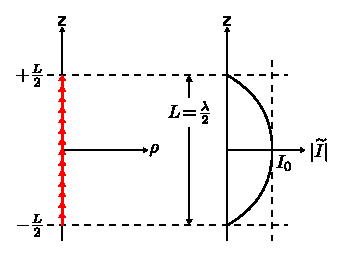
\includegraphics[width=3in]{modules/m0200_fHWD.eps} 
% https://commons.wikimedia.org/wiki/File:Current_distribution_of_the_hwd.svg
}}{Two coordinate systems. On the left, a vertical z-axis and a horizontal axis, small rho. On the right, a vertical z-axis and a horizontal axis absolute value of capital I tilde.  A dashed rectangle has height negative capital L over 2 to capital L over 2 between the two graphs. On the left graph short arrows run the length of the rectangle. On the right graph, a half-period of sine is drawn around the origin for the positive capital I subscript 0 direction.}
\end{center}
\centerline{\scriptsize 
\copyright~\hyperref[m0200_fHWD_Credit]{C.\ Wang} 
\href{https://creativecommons.org/licenses/by-sa/4.0/}{CC BY-SA 4.0} 
} % \centerline  
\caption{
\label{m0200_fHWD}
Current distribution of the half-wave dipole (HWD).
}
\end{figure}
%
This is the distribution expected on a thin straight wire having length $L=\lambda/2$, where $\lambda$ is wavelength.
This distribution is described mathematically as follows:
%
\begin{equation}
\widetilde{I}(z) \approx I_0 \cos \left( \pi \frac{z}{L} \right) ~~~ \mbox{for} ~ \left|z\right|\le\frac{L}{2}
\label{m0200_eHWD1}
\end{equation}
%
where $I_0$ (SI base units of A) is a complex-valued constant indicating the maximum magnitude of the current and its phase.
Note that the current is zero at the ends of the dipole; i.e.,
$\widetilde{I}(z) = 0$ for $\left|z\right|= L/2$.
Note also that this ``cosine pulse'' distribution is very similar to the triangular distribution of the ESD, and is reminiscent of the sinusoidal variation of current in a standing wave.
\index{standing wave}

Since $L=\lambda/2$ for the HWD, Equation~\ref{m0200_eHWD1} may equivalently be written:
%
\begin{equation}
\widetilde{I}(z) \approx I_0 \cos \left( 2\pi \frac{z}{\lambda} \right)
\label{m0200_eHWD2}
\end{equation}

The electromagnetic field radiated by this distribution of current may be calculated using the method described in Section~\ref{m0199_Radiation_from_a_Thin_Straight_Filament_of_Current}, in particular:
%
\begin{flalign}
\widetilde{\bf E}({\bf r}) &\approx \hat{\bf \theta} j \frac{\eta}{2} \frac{e^{-j\beta r}}{r}~\left(\sin\theta\right) \nonumber \\
                           & ~~~\cdot\left[\frac{1}{\lambda}\int_{-L/2}^{+L/2} \widetilde{I}(z') e^{+j\beta z'\cos{\theta}} dz'\right] \label{m0200_eESDE}
\end{flalign}
%
which is valid for field points ${\bf r}$ far from the dipole; i.e., for $r\gg L$ and $r\gg \lambda$.
For the HWD, the quantity in square brackets is
%
\begin{equation}
\frac{I_0}{\lambda}\int_{-\lambda/4}^{+\lambda/4} \cos \left( 2\pi \frac{z'}{\lambda} \right) e^{+j\beta z'\cos{\theta}} dz'
\end{equation}
%
The evaluation of this integral is straightforward, but tedious.  The integral reduces to
%
\begin{equation}
\frac{I_0}{\pi} \frac{\cos\left[\left(\pi/2\right)\cos\theta\right]}{\sin^2\theta}
\end{equation}
%
Substitution into Equation~\ref{m0200_eESDE} yields
%
\begin{equation}
\widetilde{\bf E}({\bf r}) \approx \hat{\bf \theta} j \frac{\eta I_0}{2\pi}  
  \frac{\cos\left[\left(\pi/2\right)\cos\theta\right]}{\sin\theta}
  \frac{e^{-j\beta r}}{r}
\end{equation}
%
The magnetic field may be determined from this result using Ampere's law.
However, a simpler method is to use the fact that the electric field, magnetic field, and direction of propagation $\hat{\bf r}$ are mutually perpendicular and related by:
%
\begin{equation}
\widetilde{\bf H} = \frac{1}{\eta} \hat{\bf r} \times \widetilde{\bf E}
\end{equation}
%
This relationship indicates that the magnetic field will be $+\hat{\bf \phi}$-directed.

The magnitude and polarization of the radiated field is similar to that of the electrically-short dipole (ESD; Section~\ref{m0198_Radiation_from_an_Electrically-Short_Dipole}).
A comparison of the magnitudes in any radial plane containing the $z$-axis is shown in Figure~\ref{m0200_fHWDvESD}.
%
\begin{figure} % <--- "[b!]" for first figure in section *only*; delete for 2nd and subsequent figures
\begin{center}
\pdftooltip{{  % note double braces
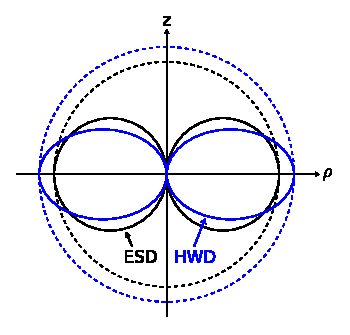
\includegraphics[width=2.5in]{modules/m0200_fHWDvESD.eps} 
% https://commons.wikimedia.org/wiki/File:Comparison_radiated_field_magnitude_of_hwd_to_esd.svg
}}{A rho-z coordinate system. There is a large dotted circle centered at the origin.  There are two smaller solid black circles within it labeled ESD centered horizontally, equal in size, tangent to each other and to the edges of the dotted circle. There is a slightly larger dotted circle also centered at the origin. There are two solid ellipses within it labeled HWD centered horizontally, equal in size tangent to each other and to the edges of the largest dotted circle.}
\end{center}
\centerline{\scriptsize 
\copyright~\hyperref[m0200_fHWDvESD_Credit]{C.\ Wang} 
\href{https://creativecommons.org/licenses/by-sa/4.0/}{CC BY-SA 4.0} 
} % \centerline  
\caption{
\label{m0200_fHWDvESD}
Comparison of the magnitude of the radiated field of the HWD to that of an electrically-short dipole also oriented along the $z$-axis.  This result is for any radial plane that includes the $z$-axis.  
}
\end{figure}
%
For either current distribution, the maximum magnitude of the fields occurs in the $z=0$ plane.
For a given terminal current $I_0$, the maximum magnitude is greater for the HWD than for the ESD.
Both current distributions yield zero magnitude along the axis of the dipole.
The polarization characteristics of the fields of both current distributions are identical.


%%%%%%%%%%%%%%%%%%%%%

{\bf Additional Reading:}
\begin{itemize}
\item ``\href{https://en.wikipedia.org/wiki/Dipole_antenna#Half-wave_dipole}{Dipole antenna}'' (section entitled ``Half-wave dipole'') on Wikipedia.
\end{itemize}

%%%%%%%%%%%%%%%%%%%%%%

\index{antenna!half-wave dipole|)}

